\chapter{回路}

NHKロボコンに出場するロボットにおいて,回路は主に図~\ref{fig:circuit_overview}に示すような範囲を担当します.図~\ref{fig:circuit_overview}~(a)にあるように,ロボットが1)~なんらかのセンサ入力を受け取り,2)~それを処理して,3)~なんらかの運動を出力するシステムであると考えたとき,回路が提供する主な機能としては a)~物理量を計算機で扱える形に処理すること,b)~計算資源を提供すること,c)~アクチュエータを駆動すること,の3点があげられます.
本章ではこの3つの機能について,ロボットの回路構成を決定する上で必要となる事項をそれぞれ解説します.
この資料は様々な回路要素を比較し,回路の視点からロボットの構成を検討することができるようになることを目的としています.
このため,各回路の動作原理等の詳細については省略いたします.
実際に実装する際には,本資料も参考にしつつ自習していただければ幸いです.

\begin{figure}[h]
  \centering
  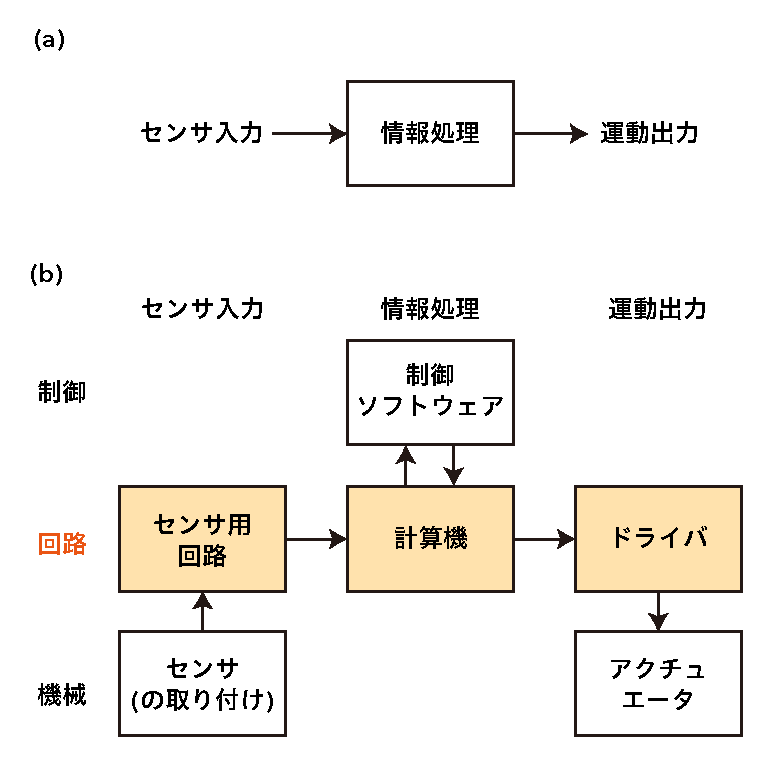
\includegraphics[width=10cm]{circuit/fig/1_circuit_overview.pdf}
  \caption{回路の視点で見たロボットの構成.(a) 大まかな構成. (b) 制御,回路,機械のレイヤに分類した場合の構成.オレンジの部分が回路の担当部分を示している.図中の矢印は主な処理の流れを表す.}
  \label{fig:circuit_overview}
\end{figure}


\section{計算機}

まず初めに,ロボットの回路構成の決定に大きく影響する計算機について説明していきます.

\subsection{計算機の種類}

NHKロボコンで用いる計算機は,図~\ref{fig:computers}のように分類でき,それぞれロボットに合わせて搭載するものを選びます.

マイコンは,計算速度は速くないものの,安価であることや入出力ピンが多数あり多くのセンサやアクチュエータを制御できること,ハードウェアの細かな制御が行いやすいといった利点があります.
ロボコンではセンサやモータなどのハードウェアを扱うため,マイコンを使用する場面が多くあります.

シングルボードコンピュータは,PCとマイコンの中間的な存在です.PCほどではないが高速なプロセッサを搭載しているため,LinuxなどのOSが動作します.
しかし,PCとは異なり入出力ピンを備えていて,ハードウェアを制御することも可能です.
価格も1万円以下で買えるなど,非常に入手しやすいものとなっています.
計算量の多い制御を行いたい場合や,USBやEthernetで通信して用いるセンサ(カメラやLiDARなど)を用いる場合,ロボットをインターネットに接続したい場合などに便利です.

そして,シングルボードコンピュータよりもさらに大きな計算資源が要求される場合は,PCを使います.
計算資源が必要である場合の他に,タブレットPCをロボットの状態を示すディスプレイとして兼用することを意図してPCをロボットに搭載するチームもいます.

以上,価格・速度や入出力端子の観点で比較をしてきましたが,この他に,計算機を選定する場合の観点としてリアルタイム性というものがあります.リアルタイム性とは,計算が決められた時間以内に完了するかどうかという性質のことを指します.
ロボットの制御では,センサを読み取り出力を変更するということを一定周期で行う必要があるため,リアルタイム性が要求されることが多いです.
計算が終了するまでの時間が保証されていないと,例えばセンサはフェンスを捉えていたのにモータの出力を変更する処理が間に合わずフェンスに衝突してしまうなどの事故が発生してしまいます.
リアルタイム性を確保するための方法としては,リアルタイムOSを用いることや,OSがない状態でハードウェアのタイマー(マイコンに内蔵されている)を用いることなどがあります.
PCやシングルボードコンピュータを一般的なOSで用いる場合は,リアルタイム性を確保することを意図してシステムが作られていないため注意が必要です.

\begin{figure}[h]
  \centering
  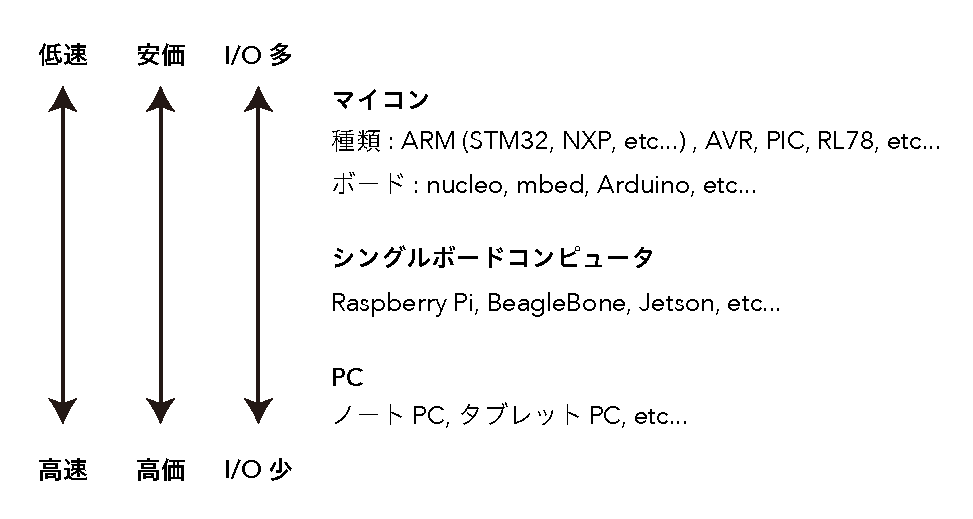
\includegraphics[width=10cm]{circuit/fig/2_computers.pdf}
  \caption{計算機の種類.}
  \label{fig:computers}
\end{figure}


\subsection{計算機まわりの回路構成}

NHKロボコンで用いる代表的な回路構成の例を図~\ref{fig:circuit_system_configuration}に示します.ロボット全体の動作を制御するソフトウェアを動かす回路として,メインボードなどと呼ばれる回路がロボットに搭載されることが多いです.メインボードに搭載されたマイコンを中心にして,ロボットの制御が行われていきます.以降,このメインボードを中心に回路の構成を説明していきます.

最も計算機の数が少ないのはマイコンを1つのみ搭載する構成です.この場合,メインボードのマイコンから直接デジタル信号またはアナログ信号を入出力してロボット全体を制御します.続いて,モータドライバやセンサ用の回路などそれぞれの回路にも1つずつマイコンを搭載するような構成もあり得ます.この場合,メインボードのマイコンは各デバイスのマイコンとシリアル通信して制御を行います.これに加えて,PCが搭載される場合もあり,メインボードのマイコンとUSBシリアル変換ICを介すなどして通信し制御を行います.メインボードと書かれている部分には,Arduinoのようなボードを用いたり,シングルボードコンピュータを用いたりすることもできます.

マイコンが1つのみの構成の利点としては,以下のような点が挙げられます.

\begin{itemize}
    \item 安価に製作できる
    \item 通信機能の開発を行わなくて良い
\end{itemize}

これらの特徴があるため,初めてロボットを製作する初心者でも扱いやすいです.一方,以下のような欠点が存在します.

\begin{itemize}
    \item ロボットに合わせてメインボードを作り替える必要がある.同じ回路を使い回すことが難しい.
    \item マイコンのピン数に限りがあるため,多くのモータやセンサを用いることが難しい.
\end{itemize}

マイコンが1つのみの構成では以上のような欠点があり,ロボットの規模が大きくなると限界を迎えます.この限界を突破するために,各デバイスにそれぞれマイコンを搭載することも多いです.図~\ref{fig:circuit_system_configuration}ではセンサ,モータドライバと区別して図示していますが,モータドライバにセンサが接続されていてモータ制御を行う構成もよくあります.このような構成ができることも,マイコンを複数搭載することの利点です.この構成の利点としては以下のような点が挙げられます.一方欠点としては,回路にかかる費用が上がることや通信機能を開発しなければならない点が挙げられます.

\begin{itemize}
    \item モジュール化して同じ回路を使いまわしやすい.通信するデータのフォーマットをうまく設計すればブラックボックスとして扱うこともできる.複数人での開発もやりやすくなる.
    \item 通信量が多すぎない限り,基板の枚数を増やすことで機能を増やせる
    \item 1つのモータに対して1つのマイコン,と言うような使い方ができるため制御周期を短くしやすい.制御の章で説明されるマイナーループを各デバイスのマイコンで高速に回し,メジャーループをメインボードと通信しつつやや長い制御周期で回すという使い方ができる.
\end{itemize}

以上に加えて,高速な計算資源が必要な場合や,カメラ等動作させるために必要なソフトウェア(ドライバ等)がPC用に提供されておりPCを搭載すれば簡単に利用できる場合など,PCやシングルボードコンピュータを追加で搭載することがあります.
これらの計算機上でリアルタイムOSを動作させることも可能であるが,リアルタイムでないLinuxなどを用いる場合はメインボードとの通信のタイミングなどに注意して開発を行う必要がある
(回路担当としては通信ができるようにハードウェアを用意するのみで,どちらかと言うとプログラムを開発する人が注意する必要がある).


\begin{figure}[h]
  \centering
  \includegraphics[width=10cm]{circuit/fig/3_systemconfiguration.pdf}
  \caption{回路の構成}
  \label{fig:circuit_system_configuration}
\end{figure}

\section{センサ}

続いて,センサについて解説します.NHKロボコンでは多くの場合センサデバイスは購入してきて使います.従って,回路担当は購入したセンサデバイスを適切な条件で動作させ,出力を処理して制御に用いることができるようにするための作業を担当します.本章では,それぞれのセンサを用いるために必要な回路について説明します.

\subsection{センサの種類}

センサには様々な種類があるが,ロボコンでしばしば用いるものとして次のセンサが挙げられます.以下,それぞれについて簡単に性質を述べた後,それぞれに必要な回路について説明します.

\begin{itemize}
    \item スイッチ
    \item 距離センサ
    \item ロータリーエンコーダ・ポテンショメータ
    \item 加速度センサ・ジャイロセンサ
    \item ラインセンサ
\end{itemize}

\subsubsection{スイッチ}

まず,最も単純なセンサとしてスイッチが挙げられます.スイッチは反応しているか,していないかの2値を返します.回路的に言えば,スイッチは電圧が高い状態か,低い状態かの2値を出力します.

スイッチには様々な種類があります.まず,機械的に金属の接点が接触したり離れたりすることによって出力が決まるスイッチとしては,コントローラなどに用いるスイッチや,リミットスイッチ(マイクロスイッチ)(Fig.~\ref{fig:circuit_switch})と呼ばれる物体をぶつけて反応させるタイプの小さなスイッチがあります.
リミットスイッチは機構の稼動範囲の両端に設置して機構を止める位置を検出する用途や,オブジェクトへの接触を検知する用途などに用います.

一方,非接触型のスイッチとして,光を利用したフォトリフレクタ(Fig.~\ref{fig:circuit_switch})や光電センサなどがあります.
これらは照射した光がフォトセンサに当たるか当たらないかによって物体の有無を検出するものです.
ものによっては反応距離を変えることができる,スイッチから少し離れた位置にあるものを検出することも可能です.
また非接触であるため壊れにくいです.
用途としては機械式スイッチと同様に機構の稼動範囲を決めたり,ロボット間で連携をする際に相手のロボットの接近を検出する用途に使います.
非接触のスイッチとしてはこの他に,磁石が近づくと反応するタイプのリードスイッチもあります.

\begin{figure}[h]
  \centering
  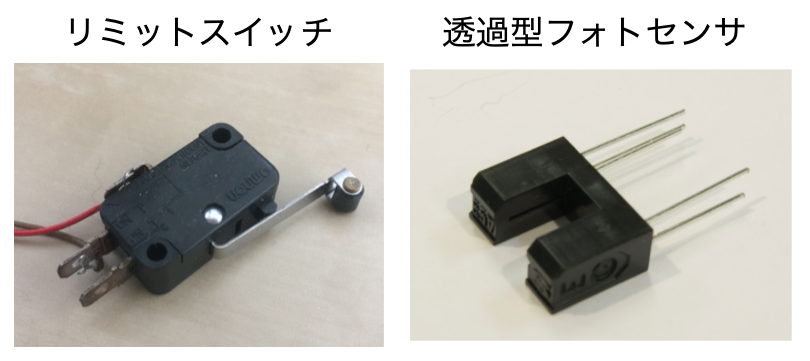
\includegraphics[width=10cm]{circuit/fig/switch.png}
  \caption{スイッチ}
  \label{fig:circuit_switch}
\end{figure}

\subsubsection{距離センサ}

フェンスやオブジェクトまでの距離を測定したい場合は距離センサを用います.自動ロボットではロボットの自己位置を推定するために用いるセンサです.距離センサとしては,超音波を用いるもの,赤外線を用いるもの(PSD距離センサ, Fig.~\ref{fig:circuit_psd}),レーザーを用いるもの(ToF方式の距離センサなど)などがあります.
出力方式には様々なものがあり,アナログ出力をするものや,シリアル通信で読み出すものなどがあります.
この他に,LiDARという2次元または3次元の距離情報を一気に読み取ることのできるセンサもあります.LiDARはPCやシングルボードコンピュータにUSBやEthernet経由でつないで用いることが多いです.

\begin{figure}[h]
  \centering
  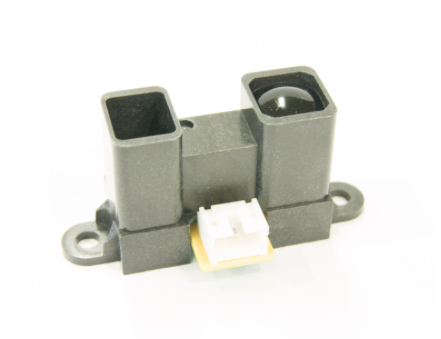
\includegraphics[width=10cm]{circuit/fig/psd.png}
  \caption{赤外線距離センサ}
  \label{fig:circuit_psd}
\end{figure}

\subsubsection{ロータリーエンコーダ・ポテンショメータ}

ロータリーエンコーダやポテンショメータ(Fig.~\ref{fig:circuit_enc})は回転角度を計測するセンサです.センサに回転軸がついていて,その軸が回された角度が分かります.
ロータリーエンコーダには,相対的な回転角度が計測できる(何度回ったか,という情報がわかるが,回転しなければ出力がない)インクリメンタル型と,絶対角度が計測できる(出力値が0度になる原点が決められていて,そこから何度回った位置にいるのかがわかる)アブソリュート型があります.ロータリーエンコーダは軸の回転に合わせて円盤が回転し光が遮られたり透過したりして回転角度を計測する光学式のものや,磁界の変化を計測して回転角度を調べる磁気式のものなどがあります.ポテンショメータは回転角度によって抵抗値が変化する,いわゆるボリュームのことです.ポテンショメータは基本的に絶対角度を出力します.
これらの回転角度センサの用途は主に2つあります.1つ目はモータに取り付けてモータ制御のためのセンサとして使うことです.モータが何度回転したかということがわかるため,位置制御や速度制御などが可能になります.2つ目は,ロボットの自己位置推定のために用いるもの(いわゆる,接地エンコーダ)です.ロボットがフィールド上のどこにいるかを調べるために,車輪を床に接地させ,その車輪の回転角度をもとにロボットが進んだ距離を計測します.

ロータリーエンコーダの出力は,一定角度回転するごとにパルス(1か0の信号)が出力される形式(2本または3本の信号線があり,それぞれA相,B相,Z相などと呼ばれます),シリアル通信で回転角度が取得できる形式などがロボコンではよく用いられます.ポテンショメータは抵抗値変化がセンサの出力ということになるため,抵抗値変化を電圧変化として読み取るための分圧回路などが必要になります.

\begin{figure}[h]
  \centering
  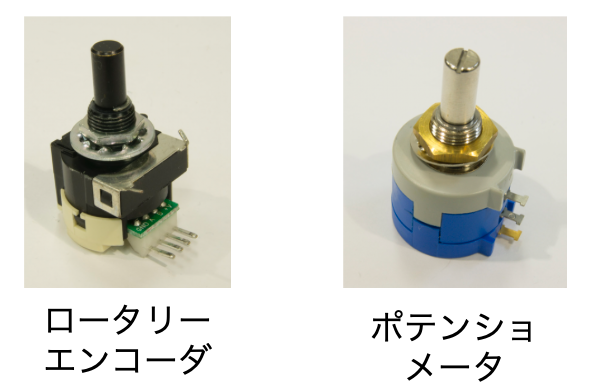
\includegraphics[width=10cm]{circuit/fig/enc.png}
  \caption{ロータリーエンコーダ・ポテンショメータ}
  \label{fig:circuit_enc}
\end{figure}

\subsubsection{加速度センサ,ジャイロセンサ}

加速度センサとジャイロセンサはまとめて慣性センサと呼ばれることもあるセンサで,加速度や角速度といった物理量を計測できます.
角速度が計測できるというとロータリーエンコーダとも似ているように感じますが,加速度センサやジャイロセンサはセンサ自体の運動が出力値として得られます.
つまり,センサをロボットに固定しておくと,ロボット全体が回転した時にその回転の速さが求められます.これらのセンサは,主に自己位置推定に用いられます.
接地エンコーダと合わせてこれらのセンサを合わせて用いることで,自己位置推定の精度を向上することが可能です.
出力は,アナログ電圧が出力されるものやシリアル通信で出力されるものなどがあります.

\subsubsection{ラインセンサ}

ラインセンサ(Fig.~\ref{fig:circuit_linesensor})は,フィールド上の白線を読み取るためのセンサーです.
フォトセンサ(明るさを測るセンサ)とLEDを組み合わせるなどして自作できます.
スキャナー用のセンサを使うチームもいます.フォトセンサの出力は,アナログ出力のものやシリアル出力のものなどがあります.

\begin{figure}[h]
  \centering
  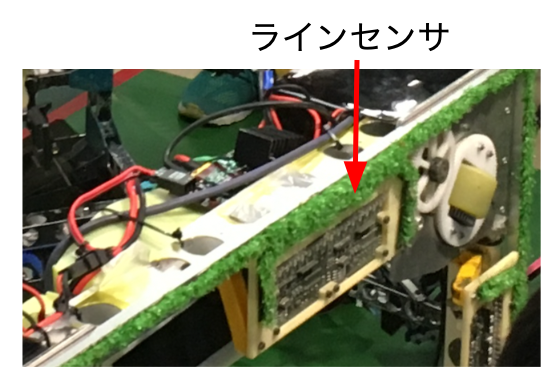
\includegraphics[width=10cm]{circuit/fig/linesensor.png}
  \caption{ラインセンサ}
  \label{fig:circuit_linesensor}
\end{figure}

\subsubsection{出力の種類}

以上センサを機能別に見てきました.
それぞれのセンサの出力方式について簡単に触れましたが,ここではそれぞれの出力方式をどのように扱ったら良いのかを説明します.
ロボコンでよく扱う出力方式には以下のものがあります.

\begin{itemize}
    \item アナログ出力(電圧)
    \item アナログ出力(抵抗値)
    \item On/Off出力
    \item シリアル出力
    \item パルス信号出力
\end{itemize}

\subsubsection{アナログ出力(電圧)}

まず1種類目は,アナログ値の電圧を出力するタイプです.アナログ値の電圧を出力するということは,例えば\SI{0}{V}から\SI{5}{V}までの範囲の電圧を計測された物理量に合わせて出力されるセンサで,ちょうど半分の大きさの計測値なら\SI{2.5}{V}が出力されるということです.
このタイプのセンサを使う場合は,A/D変換器 (analog-to-digital converter) を用いてアナログ電圧をデジタルに変換して制御に用いることが一般的です.
A/D変換器はマイコンに内蔵されておりこれを用いることが多いです.
内蔵のものであるため,比較的用いることが簡単で,新入生もよく用いる機能です.

しかし,アナログの値を使う場合はノイズの問題についての考慮が必要になる場合があります.
アナログ電圧を扱う場合は,信号にノイズが載ってしまうと,それもA/D変換されてノイズつきの値を取得してしまいます.
ロボットに使うモータは大きなノイズ源になります.このため,場合によってはノイズにより正しい値が得られず苦労することもあります.

マイコン内蔵のものより精度が高いものが利用したいとか,電源分離(モータドライバの部分で説明します)していて,マイコンとは違う電源の中の電圧が計測したいためマイコン内蔵のものでは直接測れない,というような場合に独立したA/D変換ICを用いることもあります.

\subsubsection{アナログ出力(抵抗値)}

先ほど説明したポテンショメータなどがこのタイプです.
A/D変換器で直接抵抗値を測ることはできないため,分圧回路などを使って抵抗値の変化を電圧の変化に変換してA/D変換器で読み取って使います.
分圧回路は抵抗だけからなる回路で,2つの抵抗値の比が変化すると,それぞれの抵抗にかかる電圧の比も変化することを利用して,抵抗値変化を電圧変化に変換するものです.
センサ自体に分圧回路が内蔵されていることも多いので,分圧回路を実装しないで済む場合も多いです.

\subsubsection{On/Off出力}

スイッチなどは出力が2値しかないこのタイプです.センサの中では最も単純な出力方法であると言えます.
マイコンのピンのうち,A/D変換に用いることのできるピンの数には限りがあるのですが,デジタル入力ピンは豊富にあるため,2値出力のセンサは大量に用いることができます.
ノイズの観点でも,デジタル出力なのでノイズへの耐性が高いという特性があります.
ただし,機械式スイッチではチャタリングという,OnからOffまたはOffからOnに切り替わるタイミングで出力値が素早く振動する(OnとOffを繰り返す)現象が発生してしまいます.
これは,機械的な接点が切り替わる際にバウンドして発生してしまうものです.
チャタリングがあると問題となる場合(例えば,ボタンが何回押されたかカウントする場合)は,チャタリング対策をする必要があります.詳しくは述べませんが,例えば信号線にコンデンサと抵抗からなる簡単なローパスフィルタを付けて高速な変化を抑制する,などの対策があります.

\subsubsection{シリアル出力}

1と0の信号の並びによってデータを表現し送信するのがシリアル通信です.回路的には,1を高い電圧,0を低い電圧などのようにして表現してデジタル通信を実現します(実際には他にも様々な表現方法があります).
シリアル通信にも様々な方式のものがあり,センサによってどの方式を使うかは様々です.
シリアル通信の場合は,比較的ノイズに強いです.
シリアル通信できるセンサの場合は,コマンドを送るとセンサの動作モードを変更できる,というような機能がついている場合もあります.
この時,センサそれぞれで決められたルールに従ってデータをやり取りする必要があります.
多くの場合はこれを簡単に扱うためのライブラリが配布されているため,簡単に利用することができます.
しかし,マイナーなセンサの場合などライブラリが存在しない場合があり,その時はデータシート(仕様書)を読んで自分で通信機能を実装することが必要になる場合もあります.

\subsubsection{パルス信号出力}

信号としては高い電圧と低い電圧の2値が出力されるのですが,その値が切り替わる時間間隔や回数などが計測結果を表現する,というような性質を持つものをパルス信号と言います.
インクリメンタルエンコーダのABZ相信号は一定角度変化するごとに信号の値が反転するため,これにあたります.
すなわち,速く回るほどこの切り替わりが頻繁に起こるようになり,遅く回っていると変化する時間間隔が長くなるということです.
エンコーダに関しては,このパルスをカウントする機能がマイコンに内蔵されており,それを使用してセンサを利用します.


\section{アクチュエータ}

最後に,ロボットを動かすアクチュエータについて説明します.アクチュエータそのものは,製作するメカに合わせて機械の一部としてロボットに組み込まれれます.
回路屋の仕事は,これに電流を流して動かすことです.
以下,それぞれのアクチュエータを動かす回路について簡単に説明します.

\subsection{電源分離}

各アクチュエータについて詳しく説明する前に,アクチュエータの回路において考慮しなければいけない,電源分離について紹介します.電源分離は,回路構成や電池の選定にも影響する事項です.

電源分離とは,回路をいくつかに分割し,それぞれ別の電源(主に電池)を用いて動作させることです.NHKロボコンでは,主にマイコンやセンサなどを動かす制御用回路の電源と,モータなどを駆動する駆動系電源の2つに分離することが多いでしょう.電源分離を行う理由としては,ノイズ対策や利用する電圧の違いということが挙げられます.


\subsection{エアシリンダ・ソレノイド}

エアシリンダやソレノイドは,主に直動型のアクチュエータです(回転するエアアクチュエータもあります).多くは,引っ込めている状態と伸ばした状態の2つの位置のどちらにするか,ということが制御できます.
つまり,回路的に考えれば,引っ込めるのか(Off),伸ばすのか(On)の2値のどちらかにするとか,引っ込める(引っ込めるをOn)伸ばす(伸ばすをOn)何もしない(両方Off)というようなイメージで動かしていきます.
このことからわかるように,エアシリンダやソレノイドの駆動はとてもシンプルです.
回路としては,電流を流すか,流さないかのどちらかにするようにスイッチング素子(マイコンからの信号に合わせて電流を流したり,流すのを止めたりできる回路素子)を動かせば良いだけです.
このようにシンプルであるため,比較的簡単な回路でよく,(少なくとも回路としては)コストも低くなりやすいです.

\subsection{モータ}

モータには様々な種類があるため,それぞれ分けて説明します.


\subsubsection{サーボモータ}

まず一つ目はサーボモータと言われるものです.小さな箱の中にモータと減速機,センサなどがひとまとめになって入っており,指令した角度までモータを回して止めてくれます.
回路としては,電源を繋ぎ,パルス信号を入力してそのパルスの幅を変える,ということをすれば角度を変化できます(モータドライバも中に入っているので自分で用意する必要がありません).
マイコンの電源とサーボモータの電源が同一で良い場合は,サーボモータとマイコンを繋いで,信号を送れば良いだけで回路屋としてはほとんど仕事はありません.
ただし,サーボモータの中でもパワフルなものなどは電源電圧がマイコンで使うようなものより高い場合などがあり,電源分離する場合はフォトカプラなどの部品を使って電源が違う回路にもデータが送れるようにする必要があります.
手軽に位置制御されたモータを使えるため便利です.ただし,360度以上回らないものも多く,タイヤなどには使えません.
パルス信号での制御の他に,シリアル通信により制御できるタイプもあります.


\subsubsection{ブラシモータ}

いわゆる,普通のモータです.回すにはモータドライバと言われる回路が必要です.モータドライバは既製品を買ってきて使うこともできますが,自作しているチームも多いです.モータドライバにも様々な種類があるため,それぞれについて簡単に説明します.

まず,モータを単方向に回すか,止めるかだけできるドライバが考えられます.これは,電流を流すか流さないかだけ制御できれば良いため,ソレノイドやエアシリンダと同様にOn/Offが制御できるドライバによって制御できます.非常にシンプルですが,ロボコンではほとんど使いません.

続いて,Hブリッジと呼ばれる形で4つのスイッチング素子を繋いで動かす方法があります.この回路を作ると,モータに流す電流の向きまで制御できるようになるため,両方向にモータを回せます.これを用いることが一般的です.最も単純なのは,リレーなどの素子を用いて正転,逆転,停止の3つの状態に制御できるものです.より高速にスイッチングできる素子(FETなど)を用いると,PWMをかけることによりモータの出力も変化させることができます.


\subsubsection{ブラシレスモータ}

モータが回転するにはモータ内のコイルに流れる電流の向きが回転角度に合わせて時間変化することが不可欠です.ブラシモータは,ブラシと呼ばれる部品でコイルに流れる電流の向きを変化させる仕組みになっています.これに対してブラシレスモータは,電子制御によって電流の向きを変化させることでモータを回転させる方式です.ノイズの発生が小さくできることや,効率や制御性が高いことなどの利点があります.
しかし,電流の向きを回路側で変化させなければならないため,制御することがブラシモータよりは大変です.
ドライバを自作することもできますし,ESCなどと呼ばれる既製品のドライバを買ってきて回すこともできます.
特にダクテッドファン(模型飛行機用のファン)などはブラシレスモータを使っていたりするのですが,ESCがセットで売っています.

以上様々なモータを紹介しましたが,実際の場面では自分たちの作るロボットで必要な出力をもとに,各モータの出力を比較しながら使うモータを決めていくというのが正攻法です.
力学的な計算を行って,スペック上,流しても良いとされている電流で出力できるトルクの範囲内で足りるのかなどということを検証していきます.
ただ,始めからこれらの計算をしっかりと行っていくのは大変なので,過去のロボットを見て似たような機構に使われているモータを採用してみるというのも1つの手です.


\section{その他}

その他,重要な回路素子について触れておきたいと思います.

まず1つ目が非常停止ボタンです.これはルールで付けることが義務付けられているので,必ず用意します.注意すべきなのが,モータに流す電流を全てボタンに流すとボタンが燃えてしまうことがある,という点です.ボタンの許容電流を超えそうな電流が流れることが見込まれる場合には,ボタンの状態に応じて電流が遮断できる回路を大きなリレーや大電流が流せるFETなどを用いて実装する必要があります.

続いてヒューズです.これも,安全のために取り付けます.非常停止ボタンを押さなくても,以上な大電流が流れた場合は自動で電流を遮断してくれます.非常停止用の回路とセットで考えると良いでしょう.

そして最後に,電池についても回路屋は考える必要があります.PCやスマホでも広く使われているLiPo電池を用いることが主流となっていますが,その中でも,どのぐらいの容量にするのかという点を選定することが必要になります.
電池の容量は電池がどのぐらいもつのかということだけでなく,最大で流せる電流を決定するパラメータでもあるため,おおよそどのぐらいの電流が最大で流れるのといいうことを見極めた上でそれに耐える電池を選定することが必要です.
重量が大きいパーツで,容量を大きくするほど重くなるので,出力と重量のバランスをとって選定することが重要です.
